%\mag1440
%\mag600
%\documentclass[draft,a4paper,12pt,reqno,oneside]{amsart}
%\documentclass[final,a4paper,12pt,reqno,oneside]{amsart, extarticle}
\documentclass[final,a4paper,14pt,reqno,oneside]{extarticle}
%\documentclass[draft,a4paper,12pt,reqno]{amsart}
%\documentclass[12pt]{article}
%\usepackage[T1]{fontenc}
\usepackage{cmap}
\usepackage[utf8]{inputenc}
\usepackage[T2A]{fontenc}
\usepackage[T2B]{fontenc}
\usepackage[T2C]{fontenc}
\usepackage[russian]{babel}
%\input glyphtounicode
%\pdfgentounicode=1
\usepackage{amsmath}
\usepackage{amssymb}
\usepackage{verbatim}
\usepackage{wasysym}
\usepackage{longtable}
\usepackage[center]{titlesec}
%\usepackage{sectsty}
%\usepackage{epic}
%\usepackage{eepic}
\usepackage{epsfig}
%\usepackage{floatflt}
\usepackage{graphicx}
\usepackage{amsfonts}
%\usepackage{chapterbib}
\usepackage[nottoc]{tocbibind}
\usepackage[russian]{cleveref}

%\newcommand{\crefmiddleconjunction}{, }
%\newcommand{\creflastconjunction}{ и~}
%\newcommand{\crefrangeconjunction}{--}
%\newcommand{\crefpairconjunction}{, }
\crefname{equation}{\!\!}{\!\!}
\crefname{figure}{\!\!}{\!\!}

\linespread{1.3}

\hoffset=-10mm
\textwidth=175 mm
\textheight=263 mm
\topmargin=-20 mm
\headheight=3 mm
\headsep=10 pt
\oddsidemargin=12 mm

%\setlength{\oddsidemargin}{5 mm} \setlength{\topmargin}{0 mm}
%\setlength{\headheight}{0 mm} \setlength{\headsep}{0 mm}
%\setlength{\textwidth}{160 mm} \setlength{\textheight}{240 mm}

%\tolerance=1000
%\pagestyle{empty}

\graphicspath{{./images/}}
 
\newlength{\ertp}
\unitlength 1.0mm \linethickness{0.4pt}



\renewcommand\thesection{\arabic{section}.}
\renewcommand\thesubsection{\thesection\arabic{subsection}.}
\renewcommand\thesubsubsection{\thesubsection\arabic{subsubsection}.}
%\allsectionsfont{\centering}
\begin{document}

\makeatletter
%\renewcommand{\thesection}{}
\renewcommand{\@oddhead}{}
\renewcommand{\@oddfoot}{\hfil \thepage \hfil}
\renewcommand{\l@section}{\@dottedtocline{1}{0em}{2.3em}} %содержание
%\renewcommand{\l@section}[2]{\hbox to\textwidth{#1\dotfill #2}}
\makeatother

%\renewcommand{\bibname}{Список литературы к лекции}
%\renewcommand\refname{Какой-то список}

\newcommand{\ssection}[1]{%
  \section[#1]{\centering\normalfont\scshape #1}}
\newcommand{\ssubsection}[1]{%
  \subsection[#1]{\raggedright\normalfont\itshape #1}}

\setlength{\parindent}{1.0cm}

\setlength{\leftmargini}{1.0cm}
\def\theenumi{\arabic{enumi}}
\def\labelenumi{\theenumi)}

%\setlength{\par1}{\parindent}
%\setlength{\parskip}{1ex}
%\parskip=2pt\parindent 0pt
\setlength{\ertp}{\parindent}



\renewcommand{\bibname}{СПИСОК ИСПОЛЬЗОВАННЫХ ИСТОЧНИКОВ}
\renewcommand\refname{СПИСОК ИСПОЛЬЗОВАННЫХ ИСТОЧНИКОВ}

%\input{title.tex}

%\newpage
\setcounter{page}{2}
\thispagestyle {empty}
\renewcommand{\contentsname}{\centering СОДЕРЖАНИЕ}
\tableofcontents

\newpage
\section*{ВВЕДЕНИЕ}
\addcontentsline{toc}{section}{ВВЕДЕНИЕ}


Потребность в~изучении дифракции на~различных телах очень высока. Знания, полученные путем изучения дифракции с~помощью моделей, используются как в~гидроакустике и~эхолокации, так и~в~других областях. В~дефектоскопии основной задачей является обнаружение различных включений в~однородном теле. Это позволяет проводить исследование различных объектов методом неразрушающего контроля. Задача эхолокации~--- обнаружить и~определить местоположение объектов  по~времени задержки отражённой волны.

Для~современного мира изучение простых моделей уже не~дает требуемой точности прогнозирования поведения волн. Поэтому, необходимо изучать более сложные модели, детально описывающие рассматриваемые тела и~окружающую среду. Изучение тел с~произвольно расположенными полостями является более трудной задачей, по~сравнению с~классическими моделями. 

В~настоящей работе рассматривается задача дифракции плоских звуковых волн на~упругой сфере с произвольно расположенной полостью, заполненной жидкостью, и~радиально-неоднородным упругим покрытием. С~помощью таких покрытий можно изменять звукоотражающие свойства тел, что позволяет решать различные задачи по~формированию заданной дифракционной картины. Такой слой возможно сделать в~промышленных условиях, комбинируя несколько тонких однородных слоев с~различными механическими характеристиками. В~качестве рассматриваемого тела выбрана сфера, т.к. она является подходящей аппроксимацией для~большинства сложных тел. В~ходе работы получено аналитическое описание акустического поля, рассеяного телом, предложено решение полученной краевой задачи для~системы обыкновенных дифференциальных уравнений и~представлены результаты расчетов диаграмм направленности рассеянного поля и~частотных характеристик для~различных покрытий.


\newpage
\section{МАТЕМАТИЧЕСКОЕ МОДЕЛИРОВАНИЕ РАСПРОСТРАНЕНИЯ ЗВУКОВЫХ ВОЛН}

\newpage
\subsection{Распространение звука в идеальной жидкости}

Для математического процесса моделирования распространения звука в~идеальной среде воспользуемся полной системой уравнений гидромеханики идеальной жидкости, описывающей любые движения идеальной жидкости. Эта система включает уравнение движения идеальной жидкости (уравнение Эйлера), уравнение неразрывности и~уравнение физического состояния.

Математическое описание движения жидкости осуществляется с~помощью функций, определяющих распределение скорости~$\bar{v}$, давления~$P$ и~плотности~$p$. Уравнение Эйлера имеет вид
\begin{equation}\label{eq1}
\frac{\partial \bar{v}}{\partial t} + (\bar{v} \cdot \nabla)\bar{v} = \bar F - \frac{1}{p} grad P,
\end{equation}
где $\bar F$ --- массовая сила, отнесённая к~единице массы.

Уравнение неразрывности записывается в~виде
\begin{equation}\label{eq2}
\frac{\partial \bar{p}}{\partial t} +  div (p \bar{v}) = 0.
\end{equation}

Будем считать, что движение сжимаемой жидкости происходит адиабатически. В~этом случае уравнение физического состояния принимает вид
\begin{equation}\label{eq3}
P=P_0\bigg(\frac{p}{p_0}\bigg)^\gamma, \qquad \gamma=\frac{C_P}{C_V}
\end{equation}
где $P_0$ и $p_0$ --- давление и~плотность невозмущенной жидкости; \\
 $C_P$ и $C_V$ --- теплоемкость при~постоянном давлении и~постоянном объеме.

Процесс распространения звука представляет собой малые колебания жидкости, так что в~уравнении \eqref{eq1} можно пренебречь конвективными членами. Полагая, что~внешние силы отсутствуют, получим:
\begin{equation}\label{eq4}
\frac{\partial \bar{v}}{\partial t} = - \frac{1}{p} grad P.
\end{equation}
Введем в~рассмотрение величину~$s$, называемую сжатием и~равную относительному изменению плотности
\begin{equation}\label{eq5}
s=\frac{p - p_0}{p_0}; \qquad p = p_0 (1+s).
\end{equation}

Тогда уравнение \eqref{eq3} перепишем в~виде
\begin{equation}\label{eq6}
P=P_0(1+s)^\gamma.
\end{equation}
При малых колебаниях жидкости сжатие~$s$ настолько мало, что~высшими степенями~$s$ можно пренебречь. В~результате из~выражения~\eqref{eq6} получим
\begin{equation}\label{eq7}
P=P_0(1+\gamma \cdot s).
\end{equation}

Подставим выражение~\eqref{eq5} в~уравнение неразрывности. Так как 
$$
 div(p \bar{v})= p div(\bar{v})+\bar{v}  grad p = p_0  div(\bar{v}) + p_0 s  div(\bar{v}) + \bar{v}  grad p,
$$
причем последними двумя слагаемыми можно пренебречь, то~вместо уравнения~\eqref{eq2} будем иметь
\begin{equation}\label{eq8}
\frac{\partial s}{\partial t} +  div (\bar{v}) = 0.
\end{equation}
Уравнение \eqref{eq4} в~том~же приближении сводится к~уравнению
\begin{equation}\label{eq9}
\frac{\partial \bar{v}}{\partial t} = -c^2\cdot grad s,
\end{equation}
где $c=\sqrt{\gamma \frac{P_0}{p_0}}$ --- скорость звука.

Предположим теперь, что~в~начальный момент существует потенциал скоростей~$\tilde\Psi_0$, т.е.
\begin{equation}\label{eq 10}
\bar{v}\big|_{t=0}= grad\tilde\Psi_0.
\end{equation}

Из~уравнения~\eqref{eq9} имеем
$$
\bar{v}=\bar{v}\big|_{t=0}-c^2 grad \bigg(\int\limits_{0}^{t} s d \! t\bigg).
$$
С~учетом~\eqref{eq 10} получаем
\begin{equation}\label{eq 11}
\bar{v}= grad\bigg[\tilde\Psi_0-c^2\int\limits_{0}^{t} s d \! t\bigg]= grad\tilde\Psi.
\end{equation}
Это означает, что~существует потенциал скоростей~$\tilde\Psi$ в~любой момент времени~$t:$
$$
\tilde\Psi=\tilde\Psi_0-c^2\int\limits_{0}^{t} s d \! t.
$$

Дифференцируя последнее выражение два~раза по~$t,$ получим
\begin{equation}\label{eq 12}
\frac{\partial^2\tilde\Psi}{\partial t^2}=-c^2\frac{\partial s}{\partial t}.
\end{equation}

С~другой стороны, подставляя выражение~\eqref{eq 11} в~уравнение~\eqref{eq8}, будем иметь
\begin{equation}\label{eq 13}
\frac{\partial s}{\partial t}=- div grad\tilde\Psi=-\Delta\tilde\Psi.
\end{equation}
Из~уравнений~\eqref{eq 12} и~\eqref{eq 13} приходим к~волновому уравнению
\begin{equation}\label{eq 14}
\frac{\partial^2\tilde\Psi}{\partial t^2}=c^2\Delta\tilde\Psi,
\end{equation}
которое описывает процесс распространения звука в~идеальной жидкости.

Отметим, что~знания потенциала~$\tilde\Psi$ достаточно для~определения всего процесса движения жидкости в~случае малых возмущений, так~как
$$
\bar{v}= grad\tilde\Psi;\qquad s=-\frac{1}{c^2}\frac{\partial\tilde\Psi}{\partial t}.
$$

Найдем акустическое давление~$P'=P-P_0$. Из~уравнения~\eqref{eq4}, используя приближение, сделанное для~\eqref{eq9}:
$$
\frac{\partial  grad \tilde\Psi}{\partial t} = - \frac{1}{p_0} grad P'.
$$

Занесем дифференциал под~градиент и~перенесем в~левую часть:
$$
 grad \left(\frac{\partial \tilde\Psi}{\partial t} + \frac{P'}{p_0}\right) = 0.
$$
Выражение в~скобках не~зависит от~координат. Учитывая, что~потенциал~$\tilde\Psi$ определяется с~точностью до~функции времени, приравняем выражение в~скобках нулю:
$$
\frac{\partial \tilde\Psi}{\partial t} + \frac{P'}{p_0} = 0.
$$

В~случае установившегося режима колебаний
\begin{equation}\label{eq 15}
\tilde\Psi=\Psi  e^{-i\omega t}
\end{equation}
уравнение~\eqref{eq 14} переходит в~уравнение Гельмгольца
\begin{equation}\label{eq 16}
\Delta{\Psi}+k^2\Psi=0,
\end{equation}
где $\omega$ --- круговая частота; $k=\frac{\omega}{c}$ --- волновое число.
При~этом акустическое давление 
$$
P'=-p_0 \frac{\partial \tilde\Psi}{\partial t}=-p_0 \cdot (-i \omega) \Psi  e^{-i\omega t}=ip_0\omega\tilde{\Psi}.
$$


\newpage
\subsection{Распространение звуковых волн в упругих телах}




\newpage
\section{ДИФРАКЦИЯ ЗВУКОВЫХ ВОЛН НА УПРУГОЙ СФЕРЕ, ИМЕЮЩЕЙ ПРОИЗВОЛЬНО РАСПОЛОЖЕННУЮ ПОЛОСТЬ И НЕОДНОРОДНОЕ ПОКРЫТИЕ}

\newpage
\subsection{Обзор литературы по проблеме исследования}


\newpage
\subsection{Постановка задачи}
\begin{figure}[h]
\begin{center}
\begin{minipage}[h]{0.47\linewidth}
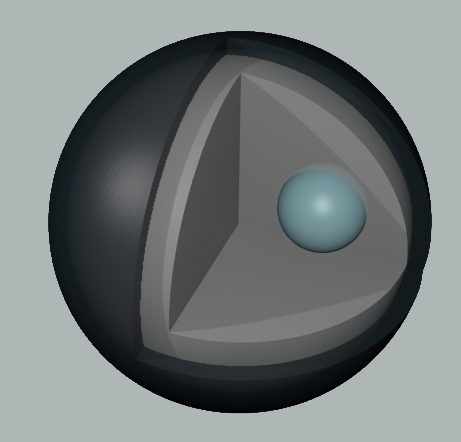
\includegraphics[width=1\linewidth]{sphere_edited.png}
\caption{<<Сфера со сферическим слоем и произвольно расположенной сферической полостью>>}\label{pic_1}
\end{minipage}
%\hfill
%\begin{minipage}[h]{0.47\linewidth}
%\includegraphics[width=1\linewidth]{2a}
%\caption{<<при $ka=3.2$>>}
%\end{minipage}
\end{center}
\end{figure}

Рассмотрим изотропный однородный упругий шар радиуса~$R_\odot$, плотность материала которого~$p_\odot$, упругие постоянные~$\lambda_\odot$ и~$\mu_\odot$, содержащий произвольно расположенную сферическую полость с~радиусом~$R_\circ$. Шар имеет покрытие в~виде неоднородного изотропного упругого слоя, внешний радиус которого равен~$R_\circledcirc$ (рис. \cref{pic_1}).
 
Свяжем с полостью тела и с~самим телом прямоугольные системы координат $x_\circ, y_\circ, z_\circ$ и $x_\odot, y_\odot, z_\odot$ соответственно так, чтобы соответствующие оси обеих систем координат были параллельны. С~декартовыми системами координат $x_\circ, y_\circ, z_\circ$ и $x_\odot, y_\odot, z_\odot$ свяжем сферические координаты $r_\circ, \theta_\circ, \varphi_\circ$ и $r_\odot, \theta_\odot, \varphi_\odot$.

Пусть модули упругости~$\lambda_\circledcirc$ и~$\mu_\circledcirc$ материала слоя описываются дифференцируемыми функциями радиальной координаты~$r_\odot$ сферической системы координат~$(r_\odot, \theta_\odot, \varphi_\odot)$, а плотность $p_\circledcirc$~--- непрерывной функцией координаты~$r_\odot$.  Окружающая тело и находящаяся в его полости жидкости~--- идеальные и однородные, имеющие плотности~$p_e, p_\circ$ и скорости звука~$c_e, c_\circ$ соответственно. 

Определим отраженные от~тела и возбужденные в~его~полости волны, а также найдем поля смещений в~упругом материале шара и неоднородном слое.


\newpage
\subsection{Аналитическое решение задачи}

Пусть из~внешнего пространства на~шар падает плоская звуковая волна. Потенциал скоростей гармонической падающей волны запишем в~виде:
\begin{equation}\label{potential speed}
\Psi_o(\bar{x}_\odot, t) = A_o \exp\left[i\left(\bar{k}_e\!\cdot\!\bar{x}_\odot-\omega t\right)\right],
\end{equation}
где $A_o$~--- амплитуда волны, \\
$\bar{k}_e$~--- волновой вектор в~окружающей жидкости,  \\
$\lvert\bar{k}_e\rvert = k_e = \omega / c_e$~--- волновое число, \\
$\bar{x}_\odot$~--- радиус-вектор, \\
$\omega$~--- круговая частота.

 Без~ограничения общности будем полагать, что волна распространяется в~направлении~$\theta_\odot = \theta_\circ = 0$. Тогда в~сферической системе координат \eqref{potential speed} запишется в~виде:
\begin{equation}\label{potential speed theta = 0}
\Psi_o(r_\odot, \theta_\odot, t) = A_o \exp\left[i\left(k_e r_\odot\cos\theta_\odot - \omega t\right)\right],
\end{equation}
В~дальнейшем временной множитель~$\exp(-i\omega t)$ будем опускать.

Разложим \eqref{potential speed theta = 0} в ряд по ортогональным функциям:
\begin{equation}
\Psi_o(r_\odot, \theta_\odot, f_\odot) = \sum\limits_{n=0}^\infty\sum\limits_{m=-n}^n {A_o}_{mn}j_n(k_e r_\odot)P_n^{\lvert m\rvert}(\cos\theta_\odot) e^{im\varphi_\odot},
\end{equation}
где $j_n(x)$~--- сферическая функция Бесселя порядка $n;$\\
$P_n^m(x)$~--- присоединенный многочлен Лежандра степени $n$ порядка $m;$\\
${A_o}_{mn} = 
\begin{cases}
A_o i^n(2n+1),& \text{при } m=0;\\
0,& \text{при } m \ne 0.
\end{cases}
$

Задача определения акустических полей вне~упругого тела и внутри его~полости в~установившемся режиме колебаний заключается в~нахождении решений уравнения Гельмгольца:
\begin{align}
\Delta\Psi_e &+ k_e^2\Psi_e = 0;\label{Helmholtz_ambient}\\
\Delta\Psi_\circ &+ k_\circ^2\Psi_\circ = 0,\label{Helmholtz_hollow}
\end{align}
где $\Psi_e$~--- потенциал скоростей полного акустического поля во~внешней среде;\\
$\Psi_\circ$~--- потенциал скоростей акустического поля в~полости тела;\\
$k_\circ = \dfrac{\omega}{c_\circ}$~--- волновое число находящейся в~полости жидкости.\\ При~этом скорости частиц жидкости и акустическое давление вне~тела и внутри полости определяются по~следующим формулам соответственно:
\begin{align}
\bar{v}_e &=  grad\Psi_e; &\quad P_e &= ip_e\omega\Psi_e;\label{eq_ven}\\
\bar{v}_\circ &=  grad\Psi_\circ; &\quad P_\circ &= ip_\circ\omega\Psi_\circ.\label{eq_vc}
\end{align}


В~силу линейной постановки задачи для $\Psi_e$ и $\Psi_o$ справедливо
\begin{equation} \label{potention_speed_ambient}
\Psi_e = \Psi_o + \Psi_s,
\end{equation}
где $\Psi_s$~--- потенциал скоростей рассеянной звуковой волны.\\
Тогда из~\eqref{Helmholtz_ambient} получаем уравнение для нахождения~$\Psi_s$:
\begin{equation} \label{Helmholtz_ambient_diffraction}
\Delta\Psi_s + k_e^2\Psi_s = 0.
\end{equation}

Из-за~произвольного расположения полости в теле потенциалы $\Psi_\circ$ и $\Psi_s$ не~будут проявлять свойства симметрии.
Уравнения~\cref{Helmholtz_hollow,Helmholtz_ambient_diffraction} запишем в~сферических системах координат~$(r_\circ, \theta_\circ, \varphi_\circ)$ и $(r_\odot, \theta_\odot, \varphi_\odot)$ соответственно:
\begin{align}
\frac1{r_\circ^2}\frac\partial{\partial r_\circ}\left(r_\circ^2 \frac{\partial\Psi_\circ}{\partial r_\circ}\right) + \frac1{r_\circ^2\sin^2\theta_\circ}\frac{\partial\Psi_\circ}{\partial\varphi_\circ^2} &+ \frac1{r_\circ^2\sin\theta_\circ}\frac\partial{\partial\theta_\circ} \left(\sin\theta_\circ \frac{\partial\Psi_\circ}{\partial\theta_\circ}\right) + k_\circ^2\Psi_\circ = 0;\\
\frac1{r_\odot^2}\frac\partial{\partial r_\odot}\left(r_\odot^2 \frac{\partial\Psi_s}{\partial r_\odot}\right) + \frac1{r_\odot^2\sin^2\theta_\odot}\frac{\partial\Psi_s}{\partial\varphi_\odot^2} &+ \frac1{r_\odot^2\sin\theta_\odot}\frac\partial{\partial\theta_\odot} \left(\sin\theta_\odot \frac{\partial\Psi_s}{\partial\theta_\odot}\right) + k_e^2\Psi_s = 0.
\end{align}

Звуковая волна в~полости тела~$\Psi_\circ$ должна удовлетворять условию ограниченности, а отраженная волна~$\Psi_s$~--- условиям излучения на~бесконечности. Поэтому потенциалы $\Psi_s$ и $\Psi_\circ$ будем искать в~виде рядов по сферическим функциям:
\begin{align}\Psi_s(r_\odot, \theta_\odot, \varphi_\odot) &= \sum\limits_{n = 0}^\infty \sum\limits_{m = -n}^n {A_s}_{mn} h_n(k_e r_\odot) P_n^{\lvert m\rvert}(\cos\theta_\odot) e^{im\varphi_\odot};\label{eq_psc}\\
\Psi_\circ(r_\circ, \theta_\circ, \varphi_\circ) &= \sum\limits_{n = 0}^\infty \sum\limits_{m = -n}^n {B_\circ}_{mn} j_n(k_\circ r_\circ) P_n^{\lvert m\rvert}(\cos\theta_\circ)e^{im\varphi_\circ},\label{eq_pc}
\end{align}
где $h_n(x)$~--- сферическая функции Ханкеля первого рода.

Распространение малых возмущений в~упругом теле для~установившегося режима движения частиц тела описывается скалярным и векторным уравнением Гельмгольца:
\begin{align}
\Delta\Psi_\odot &+ {k_\odot}_l^2\Psi_\odot = 0;\label{Helmholtz_scalar}\\
\Delta\bar{\Phi}_\odot &+ {k_\odot}_\tau^2\bar{\Phi}_\odot = 0,\label{Helmholtz_vector}
\end{align}
где ${k_\odot}_l$~--- волновое число продольных волн со~скоростью распространения \break 
${c_\odot}_l = \sqrt{\dfrac{(\lambda_\odot + 2\mu_\odot)}{p_\odot}}$;\\
${k_\odot}_\tau$~--- волновое число поперечных волн со~скоростью распространения \\
${c_\odot}_\tau = \sqrt{\dfrac{\mu_\odot}{p_\odot}}$;\\
$\Psi_\odot$ и $\bar{\Phi}_\odot$~--- скалярной и векторный потенциалы смещения соответственно.

Вектор смещения $\bar{u}_\odot$ частиц упругого тела определяется по~формуле
$$
\bar{u}_\odot =  grad \Psi_\odot +  rot \bar{\Phi}_\odot.
$$

Потенциал смещения $\Psi_\odot$ будем искать в~виде ряда по~двум локальным сферическим функциям:
\begin{equation}\label{eq_ps}
\begin{split}
\Psi_\odot = \sum\limits_{n=0}^\infty \sum\limits_{m=-n}^n 
  &{A_\odot}_{mn} h_n({k_\odot}_lr_\circ)P_n^{\lvert m\rvert}(\cos\theta_\circ) e^{im\varphi_\circ} +\\
+ &{B_\odot}_{mn} j_n({k_\odot}_lr_\odot)P_n^{\lvert m\rvert}(\cos\theta_\odot) e^{im\varphi_\odot}
\end{split}
\end{equation}

Векторный потенциал $\bar{\Phi}_\odot$ может быть представлен в~виде суммы:
$$
\bar{\Phi}_\odot = rV\bar{e}_r +  rot\bigl(rW\bar{e}_r\bigr),
$$
где $\bar{e}_r$~--- орт координатной оси~$r_\odot$ сферической системы координат~$r_\odot, \theta_\odot, \varphi_\odot,$\\
функции $V$ и $W$ удовлетворяют скалярным уравнениям Гельмгольца
\begin{align}
\Delta V &+ {k_\odot}_\tau^2 V = 0,\label{eq_V}\\
\Delta W &+ {k_\odot}_\tau^2 W = 0.\label{eq_W}
\end{align}

Компоненты вектора $\bar{u}_\odot$ выражаются через функции $\Psi_\odot, V$ и $W$ следующим образом:
\begin{equation}\label{eq_us}
\begin{split}
{u_\odot}_r &= \frac{\partial \Psi_\odot}{\partial r_\odot} - \frac{1}{r_\odot}L(W),\\
{u_\odot}_\theta &= \frac{1}{r_\odot}\frac{\partial \Psi_\odot}{\partial \theta_\odot} + \frac{1}{r_\odot}\frac{\partial}{\partial r_\odot}\left(r_\odot\frac{\partial W}{\partial \theta_\odot}\right) + \frac{1}{\sin\theta_\odot}\frac{\partial V}{\partial\varphi_\odot},\\
{u_\odot}_\varphi &= \frac{1}{r_\odot \sin\theta_\odot}\frac{\partial \Psi_\odot}{\partial \varphi_\odot} + \frac{1}{r_\odot\sin\theta_\odot}\frac{\partial}{\partial r_\odot}\left(r_\odot\frac{\partial W}{\partial \varphi_\odot}\right) - \frac{\partial V}{\partial \theta_\odot},
\end{split}
\end{equation}
где $L = \dfrac{\partial^2}{\partial\theta_\odot^2} + \ctg\theta_\odot\dfrac{\partial}{\partial\theta_\odot} + \dfrac{1}{\sin^2\theta_\odot}\dfrac{\partial^2}{\partial\varphi_\odot^2}.$

Функции $V$ и $W$ будем искать в~виде:
\begin{align}
V = \sum\limits_{n=0}^\infty \sum\limits_{m=-n}^n &{C_\odot}_{mn} h_n({k_\odot}_lr_\circ)P_n^{\lvert m\rvert}(\cos\theta_\circ) e^{im\varphi_\circ} + \notag\\
+ &{D_\odot}_{mn} j_n({k_\odot}_lr_\odot)P_n^{\lvert m\rvert}(\cos\theta_\odot) e^{im\varphi_\odot},\label{eq_v}\\
W = \sum\limits_{n=0}^\infty \sum\limits_{m=-n}^n &{E_\odot}_{mn} h_n({k_\odot}_lr_\circ)P_n^{\lvert m\rvert}(\cos\theta_\circ) e^{im\varphi_\circ} + \notag\\
+ &{F_\odot}_{mn} j_n({k_\odot}_lr_\odot)P_n^{\lvert m\rvert}(\cos\theta_\odot) e^{im\varphi_\odot}.\label{eq_w}
\end{align}

Распространение упругих волн в неоднородном слое описывается общими уравнениями движения упругой среды, которые для установившегося режима движения в сферической системе координат имеют следующий вид~\cite{Nowacki}:
\begin{equation}\label{eq_moving}
\begin{split}
\frac{\partial{\sigma_\circledcirc}_{rr}}{\partial r_\odot} &+ \frac1{r_\odot} \frac{\partial{\sigma_\circledcirc}_{r\theta}}{\partial\theta_\odot} + \frac{1}{r_\odot\sin\theta_\odot}\frac{\partial\sigma_{r\varphi}}{\partial\varphi} +\\
&+ \frac1{r_\odot}\biggl(2{\sigma_\circledcirc}_{rr}-{\sigma_\circledcirc}_{\theta\theta}-{\sigma_\circledcirc}_{\varphi\varphi}+{\sigma_\circledcirc}_{r\theta}\ctg\theta_\odot\biggr)=-p_\circledcirc\omega^2{u_\circledcirc}_r;\\
\frac{\partial{\sigma_\circledcirc}_{r\theta}}{\partial r_\odot} &+ \frac1{r_\odot} \frac{\partial{\sigma_\circledcirc}_{\theta\theta}}{\partial\theta_\odot} + \frac{1}{r_\odot\sin\theta_\odot}\frac{\partial{\sigma_\circledcirc}_{\theta\varphi}}{\partial\varphi_\odot} +\\
&+ \frac1{r_\odot}\biggl(\left({\sigma_\circledcirc}_{\theta\theta}-{\sigma_\circledcirc}_{\varphi\varphi}\right)\ctg\theta_\odot+3{\sigma_\circledcirc}_{r\theta}\biggr)\!=\!-p_\circledcirc\omega^2{u_\circledcirc}_\theta;\\
\frac{\partial{\sigma_\circledcirc}_{r\varphi}}{\partial r_\odot} &+ \frac1{r_\odot} \frac{\partial{\sigma_\circledcirc}_{\theta\varphi}}{\partial\theta_\odot} + \frac{1}{r_\odot\sin\theta_\odot}\frac{\partial{\sigma_\circledcirc}_{\varphi\varphi}}{\partial\varphi_\odot} +\\
&+ \frac1{r_\odot}\biggl(3{\sigma_\circledcirc}_{r\varphi}+2{\sigma_\circledcirc}_{\theta\varphi}\ctg\theta_\odot\biggr)=-p_\circledcirc\omega^2{u_\circledcirc}_\varphi,
\end{split}
\end{equation}
где ${u_\circledcirc}_r, {u_\circledcirc}_\theta, {u_\circledcirc}_\varphi$ --- компоненты вектора смещения $\bar{u}_\circledcirc$;\\
${\sigma_\circledcirc}_{ij}$ --- компоненты тензора напряжений неоднородной среды в сферической системе координат.

Используя связь компонентов тензора напряжений с компонентами тензора деформаций (обобщенный закон Гука), а также выражения компонентов тензора деформаций через компоненты вектора смещения~\cite{Nowacki}, получаем в сферической системе координат следующие соотношения:
\begin{equation}\label{tensor comp}
    \begin{gathered}
    \begin{aligned}
        {\sigma_\circledcirc}_{rr} &= \biggl(\lambda_\circledcirc+2\mu_\circledcirc\biggr)\frac{\partial {u_\circledcirc}_r}{\partial r_\odot} +\\
        &+ \frac{\lambda_\circledcirc} {r_\odot} \biggl(2{u_\circledcirc}_r+\frac{\partial {u_\circledcirc}_\theta}{\partial\theta_\odot}+\ctg\theta_\odot\;{u_\circledcirc}_\theta + \frac{1}{\sin\theta_\odot}\frac{\partial {u_\circledcirc}_\varphi}{\partial\varphi_\odot}\biggr);\\        
        {\sigma_\circledcirc}_{\theta\theta} &= \lambda_\circledcirc\frac{\partial {u_\circledcirc}_r}{\partial r_\odot} + \frac{2(\lambda_\circledcirc+\mu_\circledcirc)}{r_\odot} {u_\circledcirc}_r + \frac{\lambda_\circledcirc+2\mu_\circledcirc}{r_\odot} \frac{\partial {u_\circledcirc}_\theta}{\partial\theta_\odot} +\\
         &+ \frac{\lambda_\circledcirc}{r_\odot} \biggl(\ctg\theta_\odot \;{u_\circledcirc}_\theta + \frac{1}{\sin\theta_\odot}\frac{\partial {u_\circledcirc}_\varphi}{\partial\varphi_\odot}\biggr);\\
        {\sigma_\circledcirc}_{\varphi\varphi} &= \lambda_\circledcirc\frac{\partial {u_\circledcirc}_r}{\partial r_\odot} + \frac{2(\lambda_\circledcirc+\mu_\circledcirc)}{r_\odot} {u_\circledcirc}_r + \frac{\lambda_\circledcirc}{r_\odot} \frac{\partial {u_\circledcirc}_\theta}{\partial\theta_\odot} +\\
        &+ \frac{\lambda_\circledcirc+2\mu_\circledcirc}{r_\odot}\biggl(\ctg\theta_\odot \;{u_\circledcirc}_\theta + \frac{1}{\sin\theta_\odot}\frac{\partial {u_\circledcirc}_\varphi}{\partial\varphi_\odot}\biggr);\\
    \end{aligned}\\
    \begin{aligned}
        {\sigma_\circledcirc}_{r\theta}=\mu_\circledcirc&\left(\frac1{r_\odot} \frac{\partial {u_\circledcirc}_r}{\partial\theta_\odot} - \frac{{u_\circledcirc}_\theta}{r_\odot} + \frac{\partial {u_\circledcirc}_\theta}{\partial r}\right);\\
        {\sigma_\circledcirc}_{r\varphi}=\mu_\circledcirc&\left(\frac1{r_\odot\sin\theta_\odot} \frac{\partial {u_\circledcirc}_r}{\partial\varphi} - \frac{{u_\circledcirc}_\varphi}{r_\odot} + \frac{\partial {u_\circledcirc}_\varphi}{\partial r_\odot}\right);\\
        {\sigma_\circledcirc}_{\theta\varphi}=\frac{\mu_\circledcirc} {r_\odot}&\left(\frac1{\sin\theta_\odot} \frac{\partial {u_\circledcirc}_\theta}{\partial\varphi_\odot} + \frac{\partial {u_\circledcirc}_\varphi}{\partial\theta_\odot} - \ctg\theta_\odot \;{u_\circledcirc}_\varphi \right).\\
    \end{aligned}
    \end{gathered}
\end{equation}

Соотношения \eqref{tensor comp} справедливы как для однородной упругой среды, так и для неоднородного слоя. В первом случае в выражениях \eqref{tensor comp} компоненты вектора смещения $\bar{u}_\circledcirc$ и тензора напряжений $\sigma_\circledcirc,$ а также величины $\lambda_\circledcirc$ и $\mu_\circledcirc$ следует заменить на $\bar{u}_\odot, \sigma_\odot, \lambda_\odot$ и $\mu_\odot$ соответственно.

Используя эти соотношения, запишем уравнения~\eqref{eq_moving} через компоненты вектора смещения $\bar{u}_\circledcirc$:
\begin{equation*}
\begin{split}
\biggl(\lambda_\circledcirc+2\mu_\circledcirc\biggr)\frac{\partial^2 {u_\circledcirc}_r}{\partial r_\odot^2} + \frac{\mu_\circledcirc}{r_\odot^2}\frac{\partial^2 {u_\circledcirc}_r}{\partial\theta_\odot^2} +\frac{\mu_\circledcirc}{r_\odot\sin\theta_\odot}\frac{\partial^2 {u_\circledcirc}_r}{\partial\varphi_\odot^2} + \frac{\mu_\circledcirc\ctg\theta_\odot}{r_\odot^2}\frac{\partial {u_\circledcirc}_r}{\partial \theta_\odot} + \\
+ \left(\lambda_\circledcirc'+2\mu_\circledcirc'+\frac{2\lambda_\circledcirc+4\mu_\circledcirc}{r_\odot}\right)\frac{\partial{u_\circledcirc}_r}{\partial r_\odot} + \left(\frac{2\lambda_\circledcirc'}{r_\odot} - \frac{2\lambda_\circledcirc+4\mu_\circledcirc}{r_\odot^2}\right){u_\circledcirc}_r + \\
+ \frac{\lambda_\circledcirc+\mu_\circledcirc}{r_\odot}\frac{\partial^2 {u_\circledcirc}_\theta}{\partial r_\odot\partial\theta_\odot} + \frac{(\lambda_\circledcirc+\mu_\circledcirc)\ctg\theta_\odot}{r_\odot}\frac{\partial {u_\circledcirc}_\theta}{\partial r_\odot} + \\ 
+ \left(\frac{\lambda_\circledcirc'}{r_\odot} - \frac{\lambda_\circledcirc+3\mu_\circledcirc}{r_\odot^2}\right)\frac{\partial {u_\circledcirc}_\theta}{\partial \theta_\odot} +\left(\frac{\lambda_\circledcirc'\ctg\theta_\odot}{r_\odot} - \frac{(\lambda_\circledcirc+3\mu_\circledcirc)\ctg\theta_\odot}{r_\odot^2}\right){u_\circledcirc}_\theta + \\
+\frac{\lambda_\circledcirc+\mu_\circledcirc}{r_\odot\sin\theta_\odot}\frac{\partial^2 {u_\circledcirc}_\varphi}{\partial r_\odot\partial\varphi_\odot}
+ \left(\frac{\lambda_\circledcirc'}{r_\odot\sin\theta_\odot} - \frac{\lambda_\odot+3\mu_\odot}{r_\odot^2\sin\theta_\odot}\right)\frac{\partial {u_\circledcirc}_\varphi}{\partial \varphi_\odot} = -p_\circledcirc\omega^2{u_\circledcirc}_r;
\end{split}
\end{equation*}

\begin{equation*}
\begin{split}
\frac{\lambda_\circledcirc+\mu_\circledcirc}{r_\odot}\frac{\partial^2 {u_\circledcirc}_r}{\partial r_\odot \partial \theta_\odot} + \left(\frac{\mu_\circledcirc'}{r_\odot}+\frac{2\lambda_\circledcirc+4\mu_\circledcirc}{r_\odot^2}\right)\frac{\partial {u_\circledcirc}_r}{\partial \theta_\odot} + \\
+ \mu_\circledcirc \frac{\partial^2 {u_\circledcirc}_\theta}{\partial r_\odot^2} + \frac{\lambda_\circledcirc+2\mu_\circledcirc}{r_\odot^2}\frac{\partial^2 {u_\circledcirc}_\theta}{\partial \theta_\odot^2} + \frac{\mu_\circledcirc}{r_\odot^2\sin^2\theta_\odot} \frac{\partial^2 {u_\circledcirc}_\theta}{\partial \varphi^2} + \\
+ \left(\mu_\circledcirc'+ \frac{2\mu_\circledcirc}{r_\odot}\right)\frac{\partial {u_\circledcirc}_\theta}{\partial r_\odot} + \frac{(\lambda_\circledcirc+2\mu_\circledcirc)\ctg\theta_\odot}{r_\odot^2}\frac{\partial{u_\circledcirc}_\theta}{\partial \theta_\odot}-\left(\frac{\mu_\circledcirc'}{r_\odot} + \frac{\lambda_\circledcirc+2\mu_\circledcirc}{r_\odot^2\sin^2\theta_\odot}\right){u_\circledcirc}_\theta + \\
+ \frac{\lambda_\circledcirc+\mu_\circledcirc}{r_\odot^2\sin\theta_\odot}\frac{\partial^2{u_\circledcirc}_\varphi}{\partial \theta_\odot \partial \varphi_\odot} - \frac{(\lambda_\circledcirc+3\mu_\circledcirc)\ctg\theta_\odot}{r_\odot^2\sin\theta_\odot}\frac{\partial {u_\circledcirc}_\varphi}{\partial \varphi_\odot}  = -p_\circledcirc\omega^2{u_\circledcirc}_\theta;
\end{split}
\end{equation*}

\begin{equation*}
\begin{split}
\frac{\lambda_\circledcirc+\mu_\circledcirc}{r_\odot\sin\theta_\odot} \frac{\partial^2{u_\circledcirc}_r}{\partial r_\odot \partial \varphi_\odot} + \left(\frac{\mu_\circledcirc'}{r_\odot\sin\theta_\odot} + \frac{2\lambda_\circledcirc+4\mu_\circledcirc}{r_\odot^2\sin\theta_\odot} \right)\frac{\partial {u_\circledcirc}_r}{\partial \varphi_\odot} +\\
+ \frac{\lambda_\circledcirc+\mu_\circledcirc}{r_\odot^2\sin\theta_\odot}\frac{\partial^2 {u_\circledcirc}_\theta}{\partial \theta_\odot \partial \varphi_\odot} + \frac{(\lambda_\circledcirc+3\mu_\circledcirc)\ctg\theta_\odot}{r_\odot^2\sin\theta_\odot}\frac{\partial {u_\circledcirc}_\theta}{\partial \varphi_\odot} +\\
+ \mu_\circledcirc \frac{\partial^2 {u_\circledcirc}_\varphi}{\partial r_\odot^2} + \frac{\mu_\circledcirc}{r_\odot^2}\frac{\partial^2 {u_\circledcirc}_\varphi}{\partial \theta_\odot^2} + \frac{\lambda_\circledcirc+2\mu_\circledcirc}{r_\odot^2\sin^2\theta_\odot} \frac{\partial^2 {u_\circledcirc}_\varphi}{\partial \varphi_\odot^2} + \\
+ \left(\mu_\circledcirc'+\frac{2\mu_\circledcirc}{r_\odot}\right)\frac{\partial {u_\circledcirc}_\varphi}{\partial r_\odot} + \frac{\mu_\circledcirc\ctg\theta_\odot}{r_\odot^2}\frac{\partial {u_\circledcirc}_\varphi}{\partial \theta_\odot} - \left(\frac{\mu_\circledcirc'}{r_\odot} + \frac{\mu_\circledcirc}{r_\odot^2\sin^2\theta_\odot}\right){u_\circledcirc}_\varphi = - p_\circledcirc\omega^2{u_\circledcirc}_\varphi.
\end{split}
\end{equation*}
Введем новые функции ${u_\circledcirc}_2$ и ${u_\circledcirc}_3$, связанные с ${u_\circledcirc}_\theta$ и ${u_\circledcirc}_\varphi$ следующими соотношениями:
\begin{equation}\label{eq_v2v3}
{u_\circledcirc}_\theta = \dfrac{\partial {u_\circledcirc}_2}{\partial\theta_\odot} + \frac1{\sin\theta_\odot}\frac{\partial {u_\circledcirc}_3}{\partial\varphi_\odot}; \qquad {u_\circledcirc}_\varphi = \dfrac1{\sin\theta_\odot}\dfrac{\partial {u_\circledcirc}_2}{\partial\varphi_\odot} - \dfrac{\partial {u_\circledcirc}_3}{\partial\theta_\odot},
\end{equation}
запишем уравнения движения через функции ${u_\circledcirc}_r, {u_\circledcirc}_2$ и ${u_\circledcirc}_3$ и перенесем всё в левую часть:

\begin{equation}\label{eq_1.1}
\begin{split}
\biggl(\lambda_\circledcirc+2\mu_\circledcirc\biggr)\frac{\partial^2 {u_\circledcirc}_r}{\partial r_\odot^2} + \left(\lambda_\circledcirc'+2\mu_\circledcirc'+\frac{2\lambda_\circledcirc+4\mu_\circledcirc}{r_\odot}\right)\frac{\partial {u_\circledcirc}_r}{\partial r_\odot} + \frac{\mu_\circledcirc}{r_\odot^2}L({u_\circledcirc}_r) +\\
+ \left(\frac{2\lambda_\circledcirc'}{r_\odot} - \frac{2\lambda_\circledcirc+4\mu_\circledcirc}{r_\odot^2} + p_\circledcirc\omega^2\right){u_\circledcirc}_r +\\
+ \left[\frac{\lambda_\circledcirc+\mu_\circledcirc}{r_\odot}\frac{\partial}{\partial r_\odot} + \frac{\lambda_\circledcirc'}{r_\odot} - \frac{\lambda_\circledcirc+3\mu_\circledcirc}{r_\odot^2}\right]L({u_\circledcirc}_2) = 0;
\end{split}
\end{equation}
\begin{equation}\label{eq_2.1}
\begin{split}
\left[\frac{\lambda_\circledcirc+\mu_\circledcirc}{r_\odot}\frac{\partial}{\partial r_\odot}+\frac{\mu_\circledcirc'}{r_\odot}+\frac{2\lambda_\circledcirc+4\mu_\circledcirc}{r_\odot^2}\right]\frac{\partial{u_\circledcirc}_r}{\partial \theta_\odot} + \frac{\lambda_\circledcirc+2\mu_\circledcirc}{r_\odot^2}\frac{\partial}{\partial \theta_\odot}L({u_\circledcirc}_2) + \\
+ \left[\mu_\circledcirc\frac{\partial^2}{\partial r_\odot^2} + \left(\mu_\circledcirc'+\frac{2\mu_\circledcirc}{r_\odot}\right)\frac{\partial}{\partial r_\odot} - \frac{\mu_\circledcirc'}{r_\odot} + p_\circledcirc\omega^2\right]\left[\frac{\partial {u_\circledcirc}_2}{\partial\theta_\odot} + \frac{1}{\sin\theta_\odot}\frac{\partial{u_\circledcirc}_3}{\partial\varphi_\odot}\right]+\\
+ \frac{\mu_\circledcirc}{r_\odot^2\sin\theta_\odot}\frac{\partial}{\partial\varphi_\odot}L({u_\circledcirc}_3) = 0;
\end{split}
\end{equation}
\begin{equation}\label{eq_3.1}
\begin{split}
\frac{1}{r_\odot\sin\theta_\odot}\left[\biggl(\lambda_\circledcirc+\mu_\circledcirc\biggr)\frac{\partial}{\partial r_\odot} + \mu_\circledcirc' + \frac{2\lambda_\circledcirc+4\mu_\circledcirc}{r_\odot}\right]\frac{\partial {u_\circledcirc}_r}{\partial\varphi_\odot} +\\
+ \left[\mu_\circledcirc\frac{\partial^2}{\partial r_\odot^2} + \left(\mu_\circledcirc'+\frac{2\mu_\circledcirc}{r_\odot}\right)\frac{\partial}{\partial r_\odot} - \frac{\mu_\circledcirc'}{r_\odot} + p_\circledcirc\omega^2\right]\left[\frac{1}{\sin\theta_\odot}\frac{\partial {u_\circledcirc}_2}{\partial\varphi_\odot} - \frac{\partial {u_\circledcirc}_3}{\partial\theta_\odot}\right] +\\
+ \frac{\lambda_\circledcirc+2\mu_\circledcirc}{r_\odot^2\sin\theta_\odot}\frac{\partial}{\partial \varphi_\odot}L({u_\circledcirc}_2) -\frac{\mu_\circledcirc}{r_\odot^2}\frac{\partial}{\partial\theta_\odot}L({u_\circledcirc}_3) = 0,
\end{split}
\end{equation}
где $\lambda_\circledcirc' = \dfrac{ d \!\lambda_\circledcirc}{ d \! r_\odot},\quad\mu_\circledcirc' = \dfrac{ d \!\mu_\circledcirc}{ d \! r_\odot}.$

Получим преобразование системы уравнений, имеющей специальный вид. Пусть система уравнений выглядит следующим образом:
\begin{equation}\label{exaple_system}
\begin{aligned}
\frac{\partial A}{\partial \theta} + \frac{1}{\sin\theta}\frac{\partial B}{\partial\varphi} &= 0;\\
- \frac{\partial B}{\partial\theta} + \frac{1}{\sin\theta}\frac{\partial A}{\partial \varphi}  &= 0,
\end{aligned}
\end{equation}
Первое уравнение системы домножим на $\sin(\theta_\odot)$ и продифференцируем по $\theta_\odot$, а второе уравнение --- продифференцируем по $\varphi_\odot.$ Сложим полученные уравнения и разделим на $\sin(\theta_\odot)$. Получим следующее уравнение:
\begin{equation*}
L(A) = 0.
\end{equation*}
Теперь продифференцируем первое уравнение системы по $\varphi_\odot$ и вычтем второе уравнение, предварительно умноженное на $\sin(\theta_\odot)$ и продифференцированное по $\theta_\odot,$ а затем всё разделим на $\sin(\theta_\odot).$ Получим следующее уравнение:
\begin{equation*}
L(B) = 0.
\end{equation*}

Таким образом, преобразование системы \cref{exaple_system} выглядит следующим образом:
\begin{align}\label{eq_transform}
\left\{\begin{aligned}
\dfrac{\partial A}{\partial \theta} + \dfrac{1}{\sin\theta}\dfrac{\partial B}{\partial\varphi} &= 0\\
- \dfrac{\partial B}{\partial\theta} + \dfrac{1}{\sin\theta}\dfrac{\partial A}{\partial \varphi} &= 0
\end{aligned}\right. 
&& \Rightarrow && 
\left\{\begin{aligned}
L(A) &= 0\\
L(B) &= 0
\end{aligned}\right. 
\end{align}
Данное преобразование уравнений позволяет устранить связь между функциями $A$ и $B.$

Применим преобразование \cref{eq_transform} к уравнениям \cref{eq_2.1,eq_3.1}. Получим следующие уравнения:
\begin{align}
\begin{split}
\left[\frac{\lambda_\circledcirc+\mu_\circledcirc}{r_\odot}\frac{\partial}{\partial r_\odot} + \frac{\mu_\circledcirc'}{r_\odot} + \frac{2\lambda_\circledcirc+4\mu_\circledcirc}{r_\odot^2}\right]&L({u_\circledcirc}_r)+\\
\left[\mu_\circledcirc\frac{\partial^2}{\partial r_\odot^2} + \left(\mu_\circledcirc'+\frac{2\mu_\circledcirc}{r_\odot}\right)\frac{\partial}{\partial r_\odot} - \frac{\mu_\circledcirc'}{r_\odot} + p_\circledcirc\omega^2\right]&L({u_\circledcirc}_2) + \\
 + \frac{\lambda_\circledcirc+2\mu_\circledcirc}{r_\odot^2}&L^2({u_\circledcirc}_2) = 0,
\end{split}\label{eq_2.2}\\
\begin{split}
\left[\mu\frac{\partial^2}{\partial r_\odot^2} + \left(\mu_\circledcirc' + \frac{2\mu_\circledcirc}{r_\odot}\right)\frac{\partial}{\partial r_\odot} - \frac{\mu_\circledcirc'}{r_\odot} + p_\circledcirc\omega^2\right]&L({u_\circledcirc}_3) + \\
\frac{\mu_\circledcirc}{r_\odot^2}&L^2({u_\circledcirc}_3) = 0.\label{eq_3.2}
\end{split}
\end{align}

В результате получили систему, состоящую из уравнений \cref{eq_1.1,eq_2.2,eq_3.2}.

Функции ${u_\circledcirc}_r, {u_\circledcirc}_2$ и ${u_\circledcirc}_3$ также будем искать в виде разложений по сферическим функциям:
\begin{equation}\label{eq_uru2u3}
\begin{split}
{u_\circledcirc}_r(r_\odot, \theta_\odot, \varphi_\odot) = \sum\limits_{n=0}^\infty\sum\limits_{m=-n}^n U_{1mn}(r_\odot)P_n^{\lvert m\rvert}(\cos\theta_\odot) e^{im\varphi_\odot},\\
{u_\circledcirc}_2(r_\odot, \theta_\odot, \varphi_\odot) = \sum\limits_{n=0}^\infty\sum\limits_{m=-n}^n U_{2mn}(r_\odot)P_n^{\lvert m\rvert}(\cos\theta_\odot) e^{im\varphi_\odot},\\
{u_\circledcirc}_3(r_\odot, \theta_\odot, \varphi_\odot) = \sum\limits_{n=0}^\infty\sum\limits_{m=-n}^n U_{3mn}(r_\odot)P_n^{\lvert m\rvert}(\cos\theta_\odot) e^{im\varphi_\odot}.\\
\end{split}
\end{equation}

Коэффициенты ${A_s}_{mn}, {B_\circ}_{mn}, {A_\odot}_{mn}, {B_\odot}_{mn}, {C_\odot}_{mn}, {D_\odot}_{mn}, {E_\odot}_{mn}$ и $ {F_\odot}_{mn}$ разложений \cref{eq_psc,eq_ps,eq_pc,eq_v,eq_w}, а также функции $U_{1mn},U_{2mn}$ и $U_{3mn}$ из разложений \cref{eq_uru2u3} подлежат определению из граничных условий, которые заключаются в равенстве нормальных скоростей частиц упругой среды и жидкости на внешней поверхности слоя и внутренней поверхности полого шара; равенстве на них нормального напряжения и акустического давления; отсутствии на этих поверхностях касательных напряжений. На внутренней поверхности слоя при переходе через границу раздела упругих сред должны быть непрерывны составляющие вектора смещения частиц, а также нормальные и тангенциальные напряжения. Имеем:
\begin{align}
\text{при }r_\circ &= R_\circ: \quad  &  {\sigma_\odot}_{rr} &= -P_\circ,  &  {\sigma_\odot}_{r\theta} &= 0,  &  {\sigma_\odot}_{r\varphi} &= 0, \notag\\
&&  -i\omega {u_\odot}_r &= {v_\circ}_r;\label{eq_border_1.1}\\
\text{при }r_\odot &= R_\odot: \quad  &  {\sigma_\odot}_{rr} &= {\sigma_\circledcirc}_{rr},  &  {\sigma_\odot}_{r\theta} &= {\sigma_\circledcirc}_{r\theta},  &  {\sigma_\odot}_{r\varphi} &= {\sigma_\circledcirc}_{r\varphi}, &&\notag\\
&&  {u_\odot}_r &= {u_\circledcirc}_r, \quad & {u_\odot}_\theta &= {u_\circledcirc}_\theta, \quad & {u_\odot}_\varphi &= {u_\circledcirc}_\varphi;\label{eq_border_2.1}\\
\text{при }r_\odot &= R_\circledcirc: \quad  &  {\sigma_\circledcirc}_{rr} &= -P_e,  &  {\sigma_\circledcirc}_{r\theta} &= 0,  &  {\sigma_\circledcirc}_{r\varphi} &= 0, \notag\\
&&  -i\omega {u_\circledcirc}_r &= {v_e}_{r},\label{eq_border_3.1}
\end{align} 
где ${v_\circ}_r=\partial\Psi_\circ/\partial r, \quad {v_e}_r=\partial\Psi_e/\partial r$~--- радиальная компонента скорости частиц в жидкости внутри полости $\bar{v}_\circ$ и в окружающем пространстве $\bar{v}_e$ соответственно.

Используя выражения \cref{eq_ven,tensor comp,eq_v2v3}, запишем граничные условия \cref{eq_border_3.1} через функции $\Psi_o, \Psi_s, {u_\circledcirc}_r, {u_\circledcirc}_2$ и ${u_\circledcirc}_3.$ Получим для $r_\odot = R_\circledcirc:$
\begin{align}
&\biggl(\lambda_\circledcirc+2\mu_\circledcirc\biggr)\frac{\partial {u_\circledcirc}_r}{\partial r_\odot} + \frac{2\lambda_\circledcirc}{r_\odot}{u_\circledcirc}_r + \frac{\lambda_\circledcirc}{r_\odot}L({u_\circledcirc}_2) = -ip_e\omega\left(\Psi_o+\Psi_s\right);\label{eq_Rl.2}\\
\mu_\circledcirc&\frac{\partial}{\partial \theta_\odot}\left(\frac{{u_\circledcirc}_r-{u_\circledcirc}_2}{r_\odot} + \frac{\partial {u_\circledcirc}_2}{\partial r_\odot}\right) + \frac{\mu_\circledcirc}{\sin\theta_\odot}\frac{\partial}{\partial \varphi_\odot}\left(\frac{\partial {u_\circledcirc}_3}{\partial r_\odot} - \frac{{u_\circledcirc}_3}{r_\odot}\right) = 0;\label{eq_Rl.3}\\
\frac{\mu_\circledcirc}{\sin\theta_\odot}&\frac{\partial}{\partial \varphi_\odot}\left(\frac{{u_\circledcirc}_r-{u_\circledcirc}_2}{r_\odot} + \frac{\partial {u_\circledcirc}_2}{\partial r_\odot}\right) - \mu_\circledcirc\frac{\partial}{\partial \theta_\odot}\left(\frac{\partial {u_\circledcirc}_3}{\partial r_\odot} - \frac{{u_\circledcirc}_3}{r_\odot}\right) = 0;\label{eq_Rl.4}
\end{align}
\begin{equation}\label{eq_Rl.1}
-i\omega{u_\circledcirc}_r = \frac{\partial(\Psi_o+\Psi_s)}{\partial r_\odot} .
\end{equation}


Рассмотрим уравнения \cref{eq_Rl.3,eq_Rl.4}. Применим к ним преобразование \cref{eq_transform}. Получим следующие уравнения:
\begin{align}
\mu_\circledcirc \,L\!\left(\frac{{u_\circledcirc}_r-{u_\circledcirc}_2}{r_\odot} + \frac{\partial {u_\circledcirc}_2}{\partial r_\odot}\right)&\Biggr|_{r_\odot = R_\circledcirc} = 0.\label{eq_Rl.3a}\\
\mu_\circledcirc \,L\!\left(\frac{\partial {u_\circledcirc}_3}{\partial r_\odot} - \frac{{u_\circledcirc}_3}{r_\odot}\right)&\Biggr|_{r_\odot = R_\circledcirc} = 0.\label{eq_Rl.4a}
\end{align}


Аналогично, используя выражения \cref{eq_us,tensor comp,eq_v2v3}, запишем граничные условия \cref{eq_border_2.1} через функции ${u_\circledcirc}_r, {u_\circledcirc}_2, {u_\circledcirc}_3, \Psi_\odot, V$ и $W.$ Для $r_\odot = R_\odot$ получим:
\begin{align}
\begin{split}
&\biggl(\lambda_\circledcirc+2\mu_\circledcirc\biggr)\frac{\partial {u_\circledcirc}_r}{\partial r_\odot} + \frac{2\lambda_\circledcirc}{r_\odot}{u_\circledcirc}_r + \frac{\lambda_\circledcirc}{r_\odot}L({u_\circledcirc}_2) = \\
= \frac{\lambda_\odot}{r_\odot^2}&\left(\frac{\partial}{\partial r_\odot}\left(r_\odot^2\frac{\partial\Psi_\odot}{\partial r_\odot}\right)+L(\Psi_\odot)\right) + 2\mu_\odot\left(\frac{\partial^2 \Psi_\odot}{\partial r_\odot^2} - \frac{\partial}{\partial r_\odot}\left(\frac{L(W)}{r_\odot}\right)\right);
\end{split}\label{eq_Rs.1}\\
\begin{split}
\mu_\circledcirc&\frac{\partial}{\partial \theta_\odot}\left(\frac{{u_\circledcirc}_r-{u_\circledcirc}_2}{r_\odot} + \frac{\partial {u_\circledcirc}_2}{\partial r_\odot}\right) + \frac{\mu_\circledcirc}{\sin\theta_\odot}\frac{\partial}{\partial \varphi_\odot}\left(\frac{\partial {u_\circledcirc}_3}{\partial r_\odot} - \frac{{u_\circledcirc}_3}{r_\odot}\right) = \\
= 2\mu_\odot&\frac{\partial^2}{\partial r_\odot\partial\theta_\odot}\left(\frac{\Psi_\odot}{r_\odot}\right)+ \mu_\odot\frac{\partial}{\partial\theta_\odot}\left(\frac{\partial^2 W}{\partial r_\odot^2} - \frac{L(W) + 2W}{r_\odot^2} \right) + \\
+ \frac{\mu_\odot r_\odot}{\sin\theta_\odot}&\frac{\partial^2}{\partial r_\odot\partial\varphi_\odot}\left(\frac{V}{r_\odot}\right)
\end{split}\label{eq_Rs.2}\\
\begin{split}
\frac{\mu_\circledcirc}{\sin\theta_\odot}&\frac{\partial}{\partial \varphi_\odot}\left(\frac{{u_\circledcirc}_r-{u_\circledcirc}_2}{r_\odot} + \frac{\partial {u_\circledcirc}_2}{\partial r_\odot}\right) - \mu_\circledcirc\frac{\partial}{\partial \theta_\odot}\left(\frac{\partial {u_\circledcirc}_3}{\partial r_\odot} - \frac{{u_\circledcirc}_3}{r_\odot}\right) = \\
= \frac{2\mu_\odot}{\sin\theta_\odot}&\frac{\partial^2}{\partial r_\odot\partial\varphi_\odot}\left(\frac{\Psi_\odot}{r_\odot}\right)+ \frac{\mu_\odot}{\sin\theta_\odot}\frac{\partial}{\partial\varphi_\odot}\left(\frac{\partial^2 W}{\partial r_\odot^2} - \frac{L(W) + 2W}{r_\odot^2} \right) - \\
- \mu_\odot r_\odot&\frac{\partial^2}{\partial r_\odot\partial\theta_\odot}\left(\frac{V}{r_\odot}\right)
\end{split}\label{eq_Rs.3}
\end{align}
\begin{align}
{u_\circledcirc}_r &= \frac{\partial \Psi_\odot}{\partial r_\odot} - \frac{1}{r_\odot}L(W),\label{eq_Rs.4}\\
\dfrac{\partial {u_\circledcirc}_2}{\partial\theta_\odot} + \frac1{\sin\theta_\odot}\frac{\partial {u_\circledcirc}_3}{\partial\varphi_\odot} &= \frac{1}{r_\odot}\frac{\partial}{\partial \theta_\odot} \left(\Psi_\odot + \frac{\partial}{\partial r_\odot}\biggl(r_\odot W\biggr)\right) + \frac{1}{\sin\theta_\odot}\frac{\partial V}{\partial\varphi_\odot},\label{eq_Rs.5}\\
\dfrac1{\sin\theta_\odot}\dfrac{\partial {u_\circledcirc}_2}{\partial\varphi_\odot} - \dfrac{\partial {u_\circledcirc}_3}{\partial\theta_\odot} &= \frac{1}{r_\odot \sin\theta_\odot}\frac{\partial}{\partial \varphi_\odot}\left(\Psi_\odot + \frac{\partial}{\partial r_\odot}\biggl(r_\odot W\biggr)\right) - \frac{\partial V}{\partial \theta_\odot},\label{eq_Rs.6}
\end{align}

Рассмотрим уравнения \cref{eq_Rs.2,eq_Rs.3}, а также уравнения \cref{eq_Rs.5,eq_Rs.6}. Применим к ним преобразование \cref{eq_transform}. Получим следующие уравнения:
\begin{align}
\mu_\circledcirc L\!\left(\frac{{u_\circledcirc}_r-{u_\circledcirc}_2}{r_\odot} + \frac{\partial {u_\circledcirc}_2}{\partial r_\odot}\right) &= \mu_\odot L\!\left(2\frac{\partial}{\partial r_\odot}\left(\frac{\Psi_\odot}{r_\odot}\right)+  \frac{\partial^2 W}{\partial r_\odot^2} - \frac{L(W) + 2W}{r_\odot^2} \right);\label{eq_Rs.2.2}\\
\mu_\circledcirc L\!\left(\frac{\partial {u_\circledcirc}_3}{\partial r_\odot} - \frac{{u_\circledcirc}_3}{r_\odot}\right) &= \mu_\odot r_\odot\frac{\partial}{\partial r_\odot}L\!\left(\frac{V}{r_\odot}\right);\label{eq_Rs.3.2}\\
L({u_\circledcirc}_2) &= \frac{1}{r_\odot}L\!\left(\Psi_\odot + \frac{\partial}{\partial r_\odot}\biggl(r_\odot W\biggr)\right);\label{eq_Rs.5.2}\\
L({u_\circledcirc}_3) &= L(V).\label{eq_Rs.6.2}
\end{align}

Запишем граничные условия \cref{eq_border_1.1} через $\Psi_\circ, \Psi_\odot, V$ и $W,$ используя выражения \cref{eq_vc,eq_us,tensor comp}. Для $r_\circ=R_\circ$ получим:
\begin{align}
\begin{split}
\frac{\lambda_\odot}{r_\circ^2}&\left(\frac{\partial}{\partial r_\circ}\left(r_\circ^2\frac{\partial\Psi_\odot}{\partial r_\circ}\right)+L(\Psi_\odot)\right) + 2\mu_\odot\left(\frac{\partial^2 \Psi_\odot}{\partial r_\circ^2} - \frac{\partial}{\partial r_\circ}\left(\frac{L(W)}{r_\circ}\right)\right) = \\
& = - ip_\circ\omega\Psi_\circ;
\end{split}\label{eq_Rc.1}\\
\begin{split}
2\mu_\odot&\frac{\partial^2}{\partial r_\circ\partial\theta_\circ}\left(\frac{\Psi_\odot}{r_\circ}\right)+ \mu_\odot\frac{\partial}{\partial\theta_\circ}\left(\frac{\partial^2 W}{\partial r_\circ^2} - \frac{L(W) + 2W}{r_\circ^2}\right) + \\
+ \frac{\mu_\odot r_\circ}{\sin\theta_\circ}&\frac{\partial^2}{\partial r_\circ\partial\varphi_\circ}\left(\frac{V}{r_\circ}\right) = 0;
\end{split}\label{eq_Rc.2}\\
\begin{split}
\frac{2\mu_\odot}{\sin\theta_\circ}&\frac{\partial^2}{\partial r_\circ\partial\varphi_\circ}\left(\frac{\Psi_\odot}{r_\circ}\right)+ \frac{\mu_\odot}{\sin\theta_\circ}\frac{\partial}{\partial\varphi_\circ}\left(\frac{\partial^2 W}{\partial r_\circ^2} - \frac{L(W) + 2W}{r_\circ^2}\right) - \\
- \mu_\odot r_\circ&\frac{\partial^2}{\partial r_\circ\partial\theta_\circ}\left(\frac{V}{r_\circ}\right) = 0;
\end{split}\label{eq_Rc.3}
\end{align}
\begin{equation}\label{eq_Rc.4}
-i\omega \left(\frac{\partial \Psi_\odot}{\partial r_\circ} - \frac{1}{r_\circ}L(W)\right) = \frac{\partial \Psi_\circ}{\partial r_\circ}.
\end{equation}

Рассмотрим уравнения \cref{eq_Rc.2,eq_Rc.3}. Применим к ним преобразование \cref{eq_transform}. Получим следующие уравнения:
\begin{align}
\mu_\odot L\!\left(2\frac{\partial}{\partial r_\circ}\left(\frac{\Psi_\odot}{r_\circ}\right) + \frac{\partial^2 W}{\partial r_\circ^2} - \frac{L(W) + 2W}{r_\circ^2}\right)&\Biggr|_{r_\circ=R_\circ}=0;\label{eq_Rc.2.2}\\
\mu_\odot r_\circ\frac{\partial}{\partial r_\circ}L\!\left(\frac{V}{r_\circ}\right)&\Biggr|_{r_\circ=R_\circ} = 0.\label{eq_Rc.3.2}
\end{align}

Анализ уравнений движения и граничных условий позволяют утверждать, что при ${u_\circledcirc}_3 = V = 0$ будут удовлетворяться уравнения \cref{eq_V,eq_3.2}. а также граничные условия \cref{eq_Rl.4a,eq_Rs.3.2,eq_Rs.6.2,eq_Rc.3.2}, где присутствует эти функции.

Таким образом, 
$$
{C_\odot}_{mn} = {D_\odot}_{mn} = U_{3mn} = 0.
$$

Подставив разложения \cref{eq_uru2u3} в уравнения \cref{eq_1.1,eq_2.2}, воспользовавшись уравнением для присоединенных многочленов Лежандра и свойством ортогональности этих многочленов, получим для каждой пары индексов $m,n \quad(n = 0,1,\ldots; \lvert m\rvert\leq n)$ систему линейных однородных обыкновенных дифференциальных уравнений второго порядка относительно неизвестных функций \\ $U_{1mn}(r_\odot)$ и $ U_{2mn}(r_\odot):$ 
\begin{align}
\begin{split}
&(\lambda_\circledcirc + 2\mu_\circledcirc)U_{1mn}'' + \\
+ &\left(\lambda_\circledcirc'+2\mu_\circledcirc' + \frac{2\lambda_\circledcirc+4\mu_\circledcirc}{r_\odot}\right)U_{1mn}' + \left(\frac{\lambda_\circledcirc+\mu_\circledcirc}{r_\odot}\right)\bigl(-n(n+1)\bigr)U_{2mn}' + \\
+ &\left(\frac{\mu_\circledcirc}{r_\odot^2}\Bigl(-n(n+1)\Bigr) + \frac{2\lambda_\circledcirc'}{r_\odot} - \frac{2\lambda_\circledcirc + 4\mu_\circledcirc}{r_\odot^2} + p_\circledcirc\omega^2\right)U_{1mn} + \\
+ &\left(\frac{\lambda_\circledcirc'}{r_\odot} - \frac{\lambda_\circledcirc+3\mu_\circledcirc}{r_\odot^2}\right)\bigl(-n(n+1)\bigr)U_{2mn} = 0;
\end{split}\label{eq_final_1}\\
\begin{split}
&\mu_\circledcirc\bigl(-n(n+1)\bigr)U_{2mn}'' +\\
+ &\frac{\lambda_\circledcirc+\mu_\circledcirc}{r_\odot}\Bigl(-n(n+1)\Bigr)U_{1mn}' + \left(\mu_\circledcirc'+\frac{2\mu_\circledcirc}{r_\odot}\right)\bigl(-n(n+1)\bigr)U_{2mn}' + \\
+ &\left(\frac{\mu_\circledcirc'}{r_\odot} + \frac{2\lambda_\circledcirc+4\mu_\circledcirc}{r_\odot^2}\right)\bigl(-n(n+1)\bigr)U_{1mn} + \\
+ &\left(\frac{\lambda_\circledcirc+2\mu_\circledcirc}{r_\odot^2}\Bigl(-n(n+1)\Bigr) - \frac{\mu_\circledcirc'}{r_\odot} + p_\circledcirc\omega^2\right)\bigl(-n(n+1)\bigr)U_{2mn} = 0.
\end{split}\label{eq_final_2}
\end{align}

Подставим разложения \cref{eq_psc,eq_pc,eq_uru2u3} в уравнение \cref{eq_Rl.1} и выразим ${A_s}_{mn}:$
\begin{equation}\label{eq_Psc_U1}
{A_s}_{mn} = -\frac{i\omega U_{1mn}+k_e {A_o}_{mn}j_n'(k_e r_\odot)}{k_e h_n'(k_e r_\odot)}.
\end{equation}
Подставим разложения \cref{eq_psc,eq_pc,eq_uru2u3} в уравнения \cref{eq_Rl.2,eq_Rl.3a} с учетом найденного ${A_s}_{mn}$ и значения вронскиана для сферических функций Бесселя $j_n(x)h_n'(x)-j_n'(x)h_n(x)=i/x^2:$
\begin{align}
\begin{split}
&(\lambda_\circledcirc+2\mu_\circledcirc)U_{1mn}' + \left(\frac{2\lambda_\circledcirc}{r_\odot} + \frac{p_e\omega^2 h_n(k_e r_\odot)}{k_e h_n'(k_e r_\odot)}\right)U_{1mn} + \\
+& \frac{\lambda_\circledcirc}{r_\odot}\bigl(-n(n+1)\bigr)U_{2mn} 
= \frac{p_e\omega {A_o}_{mn}}{(k_e r_\odot)^2 h_n'(k_e r_\odot)};
\end{split}\\
&\mu_\circledcirc\bigl(-n(n+1)\bigr)\left(\frac{U_{1mn}-U_{2mn}}{r_\odot} + U_{2mn}'\right) = 0.
\end{align}


А используя теоремы сложения для сферических волновых функций и подставив разложения \cref{eq_uru2u3,eq_ps,eq_w} в граничные условия \cref{eq_Rs.1,eq_Rs.4,eq_Rs.2.2,eq_Rs.5.2}, найдем оставшиеся краевые условия и сможем решить  систему дифференциальных уравнений \cref{eq_final_1,eq_final_2}. После ее решения определим коэффициенты \\
${A_s}_{nm}, {B_\circ}_{nm}, {A_\odot}_{nm}, {B_\odot}_{nm}, {E_\odot}_{nm}, {F_\odot}_{nm}, {U}_{1nm}$ и ${U}_{2nm},$ разложений  \cref{eq_psc,eq_ps,eq_pc,eq_v,eq_w,eq_uru2u3} для каждой пары индексов $m,n,$ а зная коэффициенты ${A_s}_{nm}$, по формуле \cref{eq_psc} найдем акустическое поле, рассеяное упругой сферой, имеющей произвольно расположенную полость и неоднородное покрытие.

\newpage
\subsection{Решение краевой задачи для системы обыкновенных дифференциальных уравнений}

\newpage
\section{ЧИСЛЕННЫЕ ИССЛЕДОВАНИЯ}

\newpage
\subsection{Диаграмма направленности}

\newpage
\subsection{Частотные характеристики}

\newpage
\section*{ЗАКЛЮЧЕНИЕ}
\addcontentsline{toc}{section}{ЗАКЛЮЧЕНИЕ}



\newpage
\section*{ЛИТЕРАТУРА}
\addcontentsline{toc}{section}{ЛИТЕРАТУРА}



\newpage
\section*{ПРИЛОЖЕНИЯ}
\addcontentsline{toc}{section}{ПРИЛОЖЕНИЯ}


\end{document}
